\documentclass[a4paper,10pt,twocolumn]{article}
\usepackage[left=17mm,right=17mm,top=27mm,bottom=20mm,columnsep=7mm]{geometry}
\usepackage[T1]{fontenc}
\usepackage{newtxtext}
\renewcommand{\ttdefault}{lmtt}
\usepackage{amsmath}
\usepackage{newtxmath}
\usepackage{microtype}
\usepackage{graphicx}
\usepackage{booktabs,tabularx}
\usepackage{siunitx}
\usepackage{tikz}
\usetikzlibrary{arrows.meta,positioning}
\usepackage[hidelinks,bookmarks=false]{hyperref}
\usepackage{balance}
\usepackage{titlesec}
\usepackage[font=footnotesize,labelfont=bf,labelsep=period,
 justification=justified,singlelinecheck=false]{caption}
\setlength{\parindent}{1em}
\setlength{\parskip}{0pt}
\setlength{\textfloatsep}{8pt plus 2pt minus 2pt}
\setlength{\floatsep}{7pt plus 2pt minus 2pt}
\renewcommand{\dbltopfraction}{0.9}
\renewcommand{\topfraction}{0.9}
\renewcommand{\textfraction}{0.05}
\renewcommand{\figurename}{Fig.}
\titleformat{\section}{\normalfont\normalsize\bfseries}{\thesection.}{0.5em}{}
\titleformat{name=\section,numberless}{\normalfont\normalsize\bfseries}{}{0pt}{}
\titleformat{\subsection}{\normalfont\normalsize\bfseries}{\thesubsection.}{0.5em}{}
\titlespacing*{\section}{0pt}{1.2\baselineskip}{0.45\baselineskip}
\titlespacing*{\subsection}{0pt}{0.8\baselineskip}{0.15\baselineskip}
\newcommand{\StudyCaseCount}{3}
\newcommand{\StudySpectrumCount}{17}
\newcommand{\MareRange}{0.40--25.80}
\newcommand{\MareBandCount}{5}
\newcommand{\MareBands}{0.58, 0.66, 0.96, 2.72, 12.84}
\newcommand{\MareNominalRMSE}{1.03}
\newcommand{\MareCombinedRMSE}{5.20}
\newcommand{\MareGreedyGap}{-0.19}
\newcommand{\LongwaveRange}{0.40--40.00}
\newcommand{\LongwaveBandCount}{8}
\newcommand{\LongwaveBands}{0.96, 1.22, 2.94, 7.74, 8.34, 12.70, 14.92, 28.10}
\newcommand{\LongwaveNominalRMSE}{1.16}
\newcommand{\LongwaveCombinedRMSE}{2.67}
\newcommand{\LongwaveGreedyGap}{-0.08}
\newcommand{\AllGroupsRange}{0.40--24.80}
\newcommand{\AllGroupsBandCount}{8}
\newcommand{\AllGroupsBands}{0.54, 0.96, 1.30, 2.94, 6.14, 8.06, 12.62, 15.46}
\newcommand{\AllGroupsNominalRMSE}{2.64}
\newcommand{\AllGroupsCombinedRMSE}{4.52}
\newcommand{\AllGroupsGreedyGap}{-0.02}


\begin{document}
\raggedbottom
\twocolumn[{
\begin{center}
 {\fontsize{14pt}{17pt}\selectfont\bfseries
 Information-Theoretic Spectral Baseline Design for In-Situ Lunar Resource Mapping\par}
 \vspace{5mm}
 {\fontsize{10pt}{12pt}\selectfont Jakub LE\'S$^{1)}$ and Manfred GAWLAS$^{2)}$\par}
 \vspace{3mm}
 {\fontsize{8pt}{10pt}\selectfont\itshape
 $^{1)}$University of Wroclaw and Creotech Instruments S.A., Poland\par
 $^{2)}$Wroclaw University of Science and Technology, Poland\par}
\end{center}
\vspace{5mm}
\begin{center}
\begin{minipage}{\dimexpr\textwidth-60mm\relax}
\fontsize{9pt}{11.5pt}\selectfont\noindent
Compact lunar resource-mapping instruments require a defensible choice of spectral channels before detailed optical design. This study turns laboratory spectra into simple instrumentation baselines using wavelength-dependent response functions, three stated noise-sensitivity levels, and greedy D-optimal band selection. Seventeen priority minerals are represented in three configurations: a five-band mare-resource example, a long-wave-supported resource set, and seven functional groups covering all selected minerals. Every configuration is restricted to common measured spectral support; no spectrum is extrapolated. Band-count and minimum-spacing sweeps expose design sensitivity, while a small genetic search checks the greedy result. Non-negative unmixing of simulated mixtures supplies an empirical uncertainty test. Nominal abundance root-mean-square errors are \MareNominalRMSE, \LongwaveNominalRMSE, and \AllGroupsNominalRMSE\ percentage points for the three reference configurations, rising to \MareCombinedRMSE, \LongwaveCombinedRMSE, and \AllGroupsCombinedRMSE\ under combined noise, calibration-shift, and continuum-mismatch stress. The results define reproducible laboratory-domain baselines, not flight-instrument performance predictions. Thermal radiance, particulate mixing, spatial detectability, and environmental spectral variability remain explicit limitations.
\end{minipage}
\end{center}
\vspace{5mm}
\begin{center}
 {\fontsize{9pt}{11pt}\selectfont\textbf{Key Words:}\enspace
 Lunar spectroscopy; resource mapping; band selection; optimal design; spectral unmixing\par}
\end{center}
\vspace{6mm}
}]

\section*{Nomenclature}
\begingroup\fontsize{8pt}{9.5pt}\selectfont
\setlength{\tabcolsep}{0pt}\renewcommand{\arraystretch}{1.02}
\begin{tabularx}{\columnwidth}{@{}>{$}l<{$}@{\quad:\quad}X@{}}
E(\lambda) & endmember response vector\\
R_b(\lambda) & response of band $b$\\
\sigma_b & assumed standard deviation in band $b$\\
\mathbf v_b & noise-whitened spectral contrast\\
\mathcal B & selected band set\\
F(\mathcal B) & Fisher information matrix\\
\Phi(\mathcal B) & regularised log-determinant objective\\
n & number of selected bands\\
s & minimum-spacing factor\\
\mathbf a,\hat{\mathbf a} & true and estimated mixture weights\\
\end{tabularx}
\endgroup

\section{Introduction}

Lunar resource mapping joins two different questions: which materials are scientifically or operationally important, and which measurements are sufficient to distinguish them. A hyperspectral instrument can postpone the second decision, but mass, data rate, detector technology, and thermal design often favour a smaller set of channels. The required channels depend on the minerals grouped together, their host material, spectral resolution, noise, and the abundance problem to be solved. A single universal list is therefore not expected.

The Moon Mineralogy Mapper (M3) demonstrated calibrated imaging spectroscopy from 0.43 to \SI{3.0}{\micro\metre}, with signal-to-noise ratios above 400 and 100 for specified equatorial and polar reference radiances, respectively \cite{green2011m3}. Thermal instruments obey different physics. Diviner uses separate reflected-solar and emitted-radiance channels \cite{paige2010diviner}, while the proposed MIRORES concept specifically targets strong ore-mineral structure from 20 to \SI{40}{\micro\metre} with approximately 0.6--\SI{1.2}{\micro\metre} resolution \cite{ciazela2023mirores}. A baseline spanning these regimes must therefore be treated as a design sensitivity study, not as one already calibrated instrument.

The present study combines D-optimal greedy selection, multiple mineral groupings, response and noise models, and an initial unmixing uncertainty check in three deliberately small cases. Its contribution is the reproducible method and the comparison between configurations. It does not claim an optimal flight payload or physical retrieval accuracy.

\section{Spectral data and study cases}

The input is the existing RELAB collection \cite{pieters2004relab}. The selected files combine bidirectional VNIR and Fourier-transform infrared laboratory measurements. Each file is parsed using its recorded wavelength coordinate, and its checksum and support accompany the results. Interpolation outside measured support is prohibited. This matters because silently extending the last value would create flat, artificial FIR spectra and potentially artificial selected bands.

Table~\ref{tab:cases} defines the three cases. The mare-resource case uses a fixed mare matrix with ilmenite, troilite, and apatite. The long-wave case includes only samples measured through \SI{40}{\micro\metre}. The final case uses seven functional composites to include all 17 selected minerals without pretending that fewer than ten bands can independently retrieve 17 abundances. Composite members are averaged with the fixed weights in the public configuration.

\begin{table*}[t]
\caption{Configurations used in the study. The upper wavelength is set by common measured support, not by extrapolation.}
\label{tab:cases}
\centering\footnotesize
\begin{tabularx}{\textwidth}{@{}lclX@{}}
\toprule
Case & Components & Range (\si{\micro\metre}) & Content\\
\midrule
Mare resources & 4 & \MareRange & Mare matrix (anorthite, pigeonite, orthopyroxene, fayalite), ilmenite, troilite, apatite\\
Long-wave resources & 6 & \LongwaveRange & Mare matrix, ilmenite, pyrite, magnetite, apatite, sulfate assemblage\\
All priority groups & 7 & \AllGroupsRange & Oxides/oxyhydroxide, sulfides, mafic silicates, feldspar, phosphate, sulfates, silica\\
\bottomrule
\end{tabularx}
\end{table*}

The laboratory quantity is reflectance. Beyond the solar-reflected regime, an orbital instrument principally measures thermally emitted radiance; for an opaque isothermal surface, emissivity contrast is related to reflectance contrast, but temperature and viewing geometry remain necessary for an actual radiance prediction. The current work therefore optimises measured laboratory contrast only. This boundary is retained throughout the interpretation.

\section{Method}

Figure~\ref{fig:method} summarises the complete method. The same steps are applied without case-specific tuning.

\begin{figure*}[t]
\centering
\resizebox{\textwidth}{!}{%
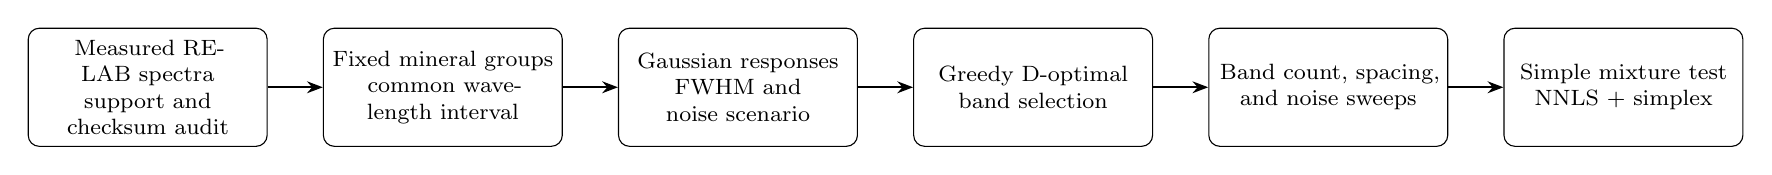
\begin{tikzpicture}[
 node distance=7mm,
 box/.style={draw,rounded corners,align=center,text width=28mm,minimum height=15mm,font=\footnotesize},
 arrow/.style={-{Stealth[length=2mm]},thick}]
\node[box] (data) {Measured RELAB spectra\\support and checksum audit};
\node[box,right=of data] (group) {Fixed mineral groups\\common wavelength interval};
\node[box,right=of group] (sensor) {Gaussian responses\\FWHM and noise scenario};
\node[box,right=of sensor] (select) {Greedy D-optimal\\band selection};
\node[box,right=of select] (test) {Band count, spacing,\\and noise sweeps};
\node[box,right=of test] (unmix) {Simple mixture test\\NNLS + simplex};
\draw[arrow] (data)--(group);
\draw[arrow] (group)--(sensor);
\draw[arrow] (sensor)--(select);
\draw[arrow] (select)--(test);
\draw[arrow] (test)--(unmix);
\end{tikzpicture}
}
\caption{Study method. All reported bands begin with measured spectral support. The genetic search is used only as a small audit of the selected reference configurations.}
\label{fig:method}
\end{figure*}

\subsection{Response and noise sensitivity}

For component $k$ and candidate band $b$, the band response is
\begin{equation}
 E_{bk}=\frac{\int R_b(\lambda)e_k(\lambda)\,d\lambda}
 {\int R_b(\lambda)\,d\lambda},\qquad
 R_b(\lambda)=\exp\!\left[-\frac{(\lambda-\lambda_b)^2}{2\tau_b^2}\right],
\end{equation}
where $\tau_b=\mathrm{FWHM}_b/(2\sqrt{2\ln2})$. Candidate centres are separated by \SI{0.02}{\micro\metre}. The adopted FWHM is \SI{0.01}{\micro\metre} below \SI{3}{\micro\metre}, increases from 0.05 to \SI{0.40}{\micro\metre} between 3 and \SI{20}{\micro\metre}, and from 0.6 to \SI{1.2}{\micro\metre} between 20 and \SI{40}{\micro\metre}. These are three transparent regimes, not a detailed common optical design.

Three signal-to-noise profiles are evaluated. Optimistic/reference/stressed SNR values are 400/200/100 in the VNIR, 200/100/50 in the MIR, and 100/50/20 in the FIR. M3 brackets the VNIR endpoints \cite{green2011m3}; the other values are sensitivity assumptions because radiance, temperature, and detector design are not yet fixed. At each candidate, $\sigma_b$ is the median component magnitude, with a 0.05 floor, divided by the stated SNR.

\subsection{D-optimal selection and spacing}

Mixture weights sum to one, so only $K-1$ component contrasts are independent. With the last component as reference, the whitened vector is
\begin{equation}
 \mathbf v_b=\frac{E_{b,1:K-1}-E_{b,K}}{\sigma_b}.
\end{equation}
For selected set $\mathcal B$, the regularised information objective is
\begin{equation}
 \Phi(\mathcal B)=\log\det\!\left(I+\sum_{b\in\mathcal B}\mathbf v_b\mathbf v_b^{\mathsf T}\right).
\end{equation}
The greedy algorithm adds the feasible band giving the largest marginal gain. Log-determinant information is a standard optimal-design criterion \cite{silvey1980optimal}; under a cardinality-only constraint, the positive-semidefinite sum gives a monotone submodular objective and the usual greedy bound applies \cite{nemhauser1978submodular,krause2008sensor}. The engineering spacing constraint changes that feasible family, so the simple cardinality guarantee is not claimed for the constrained result.

Adjacent filters are controlled by
\begin{equation}
 |\lambda_i-\lambda_j|\geq \frac{s}{2}
 (\mathrm{FWHM}_i+\mathrm{FWHM}_j).
\end{equation}
The sweep uses $s=1,2,4$: non-overlapping half-maximum intervals and two progressively conservative separations. Band counts of 4, 5, 6, 8, and 10 are tested. A small deterministic genetic search \cite{holland1975adaptation}, initialised with the greedy design, uses the identical objective and constraints for each reference case. It is an empirical check, not proof of global optimality.

\subsection{Uncertainty and mixture check}

The unregularised contrast information $F=V^{\mathsf T}V$ exposes rank directly. If $n<K-1$, independent mixture coefficients cannot be identified and linearised uncertainty is reported as unbounded. Otherwise the mean square root of $\operatorname{diag}(F^{-1})$ is used only to compare configurations.

For an easier end-to-end interpretation, 300 fixed-seed mixtures are drawn from host-weighted Dirichlet distributions. Gaussian noise is added and abundances are estimated with non-negative least squares \cite{lawson1995least}, followed by projection onto the unit simplex \cite{duchi2008projection}. Three tests are retained: nominal; a calibration case with $0.1$ FWHM band-centre scatter and 2\% continuum mismatch; and a combined case using stressed noise, $0.25$ FWHM scatter, and 5\% mismatch. The continuum term is a generic modelling perturbation, not a physical space-weathering or grain-size model.

\section{Results}

Figure~\ref{fig:designs} shows the three selected reference designs. The five-band mare case provides the compact baseline, while the two more complex groupings use eight bands. Selected centres are listed in Table~\ref{tab:results}; exact values for every sweep point are supplied as CSV.

\begin{figure*}[t]
\centering
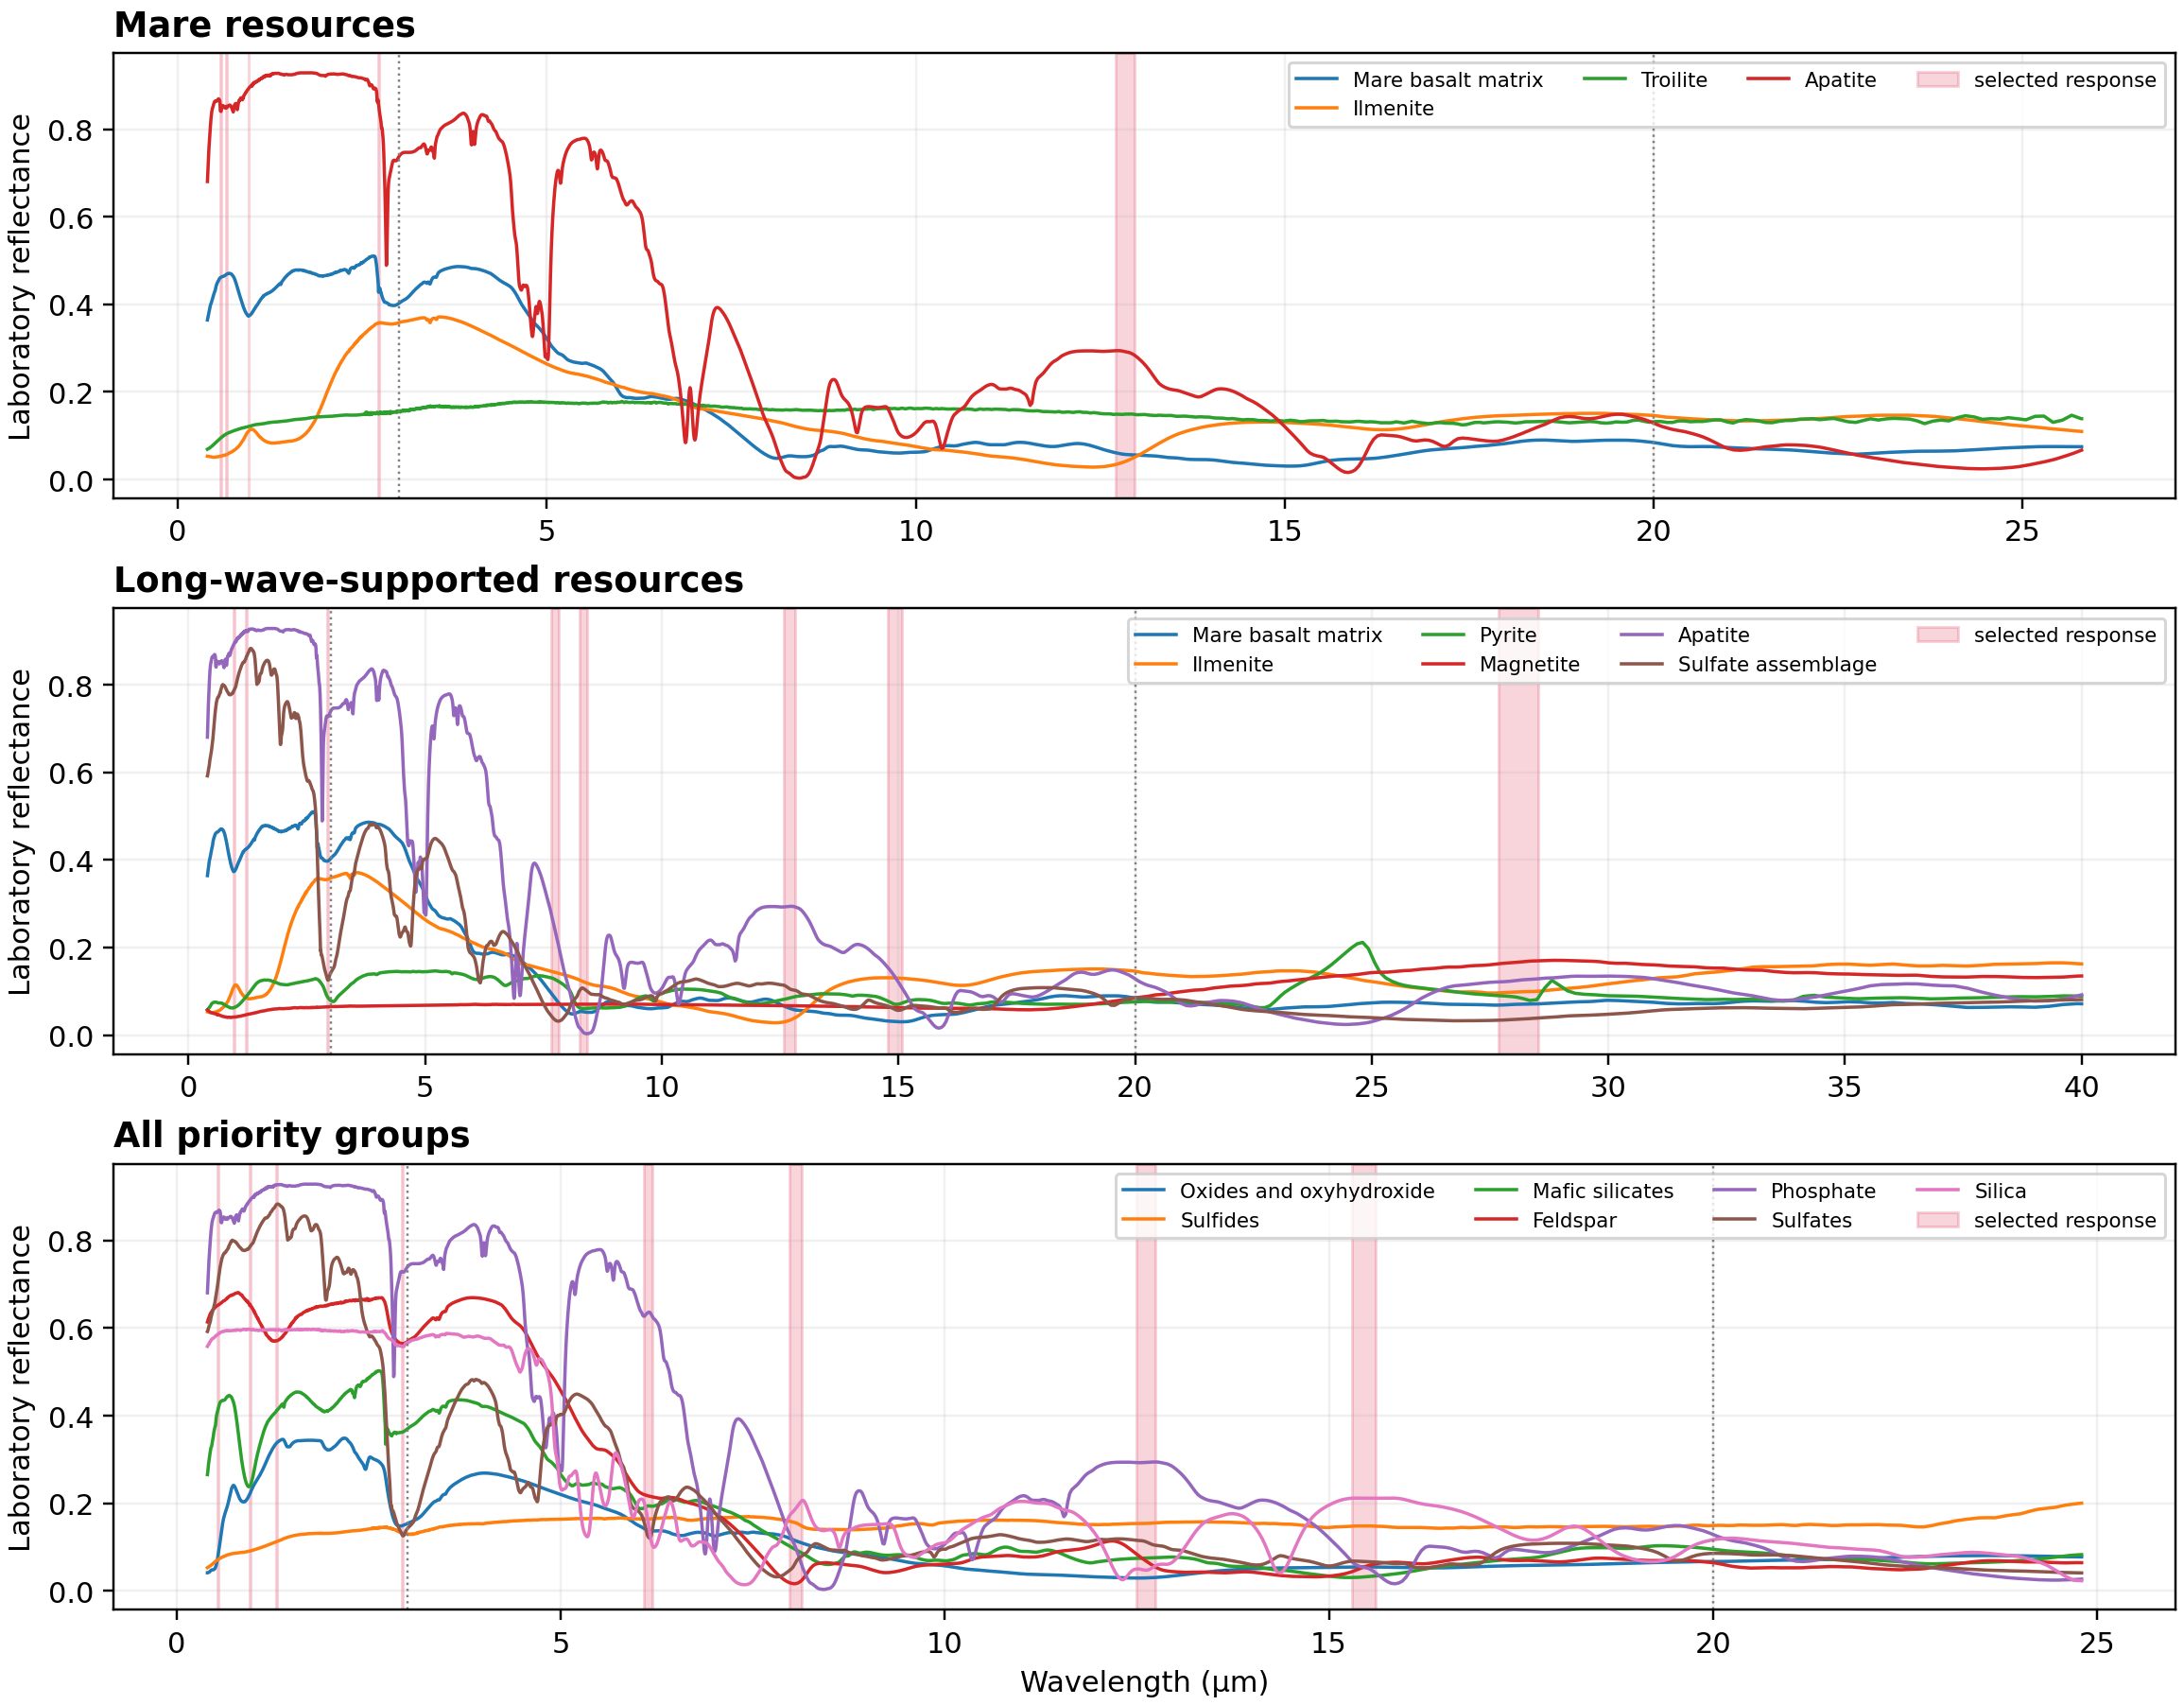
\includegraphics[width=\textwidth]{../outputs/figures/three_case_designs.png}
\caption{Measured component spectra and selected reference bands. Shaded widths show the adopted Gaussian FWHM. The first and third cases stop near \SI{25}{\micro\metre} because at least one constituent spectrum stops there; only the supported subset is extended to \SI{40}{\micro\metre}.}
\label{fig:designs}
\end{figure*}

\begin{table*}[t]
\caption{Reference configurations and empirical abundance errors. RMSE values are percentage points across all components and 300 mixtures.}
\label{tab:results}
\centering\footnotesize
\begin{tabularx}{\textwidth}{@{}lclXrr@{}}
\toprule
Case & Bands & Range (\si{\micro\metre}) & Band centres (\si{\micro\metre}) & Nominal RMSE & Combined RMSE\\
\midrule
Mare resources & \MareBandCount & \MareRange & \MareBands & \MareNominalRMSE\% & \MareCombinedRMSE\%\\
Long-wave resources & \LongwaveBandCount & \LongwaveRange & \LongwaveBands & \LongwaveNominalRMSE\% & \LongwaveCombinedRMSE\%\\
All priority groups & \AllGroupsBandCount & \AllGroupsRange & \AllGroupsBands & \AllGroupsNominalRMSE\% & \AllGroupsCombinedRMSE\%\\
\bottomrule
\end{tabularx}
\end{table*}

Increasing band count reduces linearised uncertainty in all cases (Fig.~\ref{fig:sensitivity}, left), but the improvement is not uniform. Four bands are sufficient for full rank in the four-component mare case. The six-component case requires at least five, and the seven-group case at least six. Designs below these limits may still classify spectra but cannot uniquely estimate every independent weight in this linear model.

\begin{figure*}[t]
\centering
\begin{minipage}[t]{0.49\textwidth}
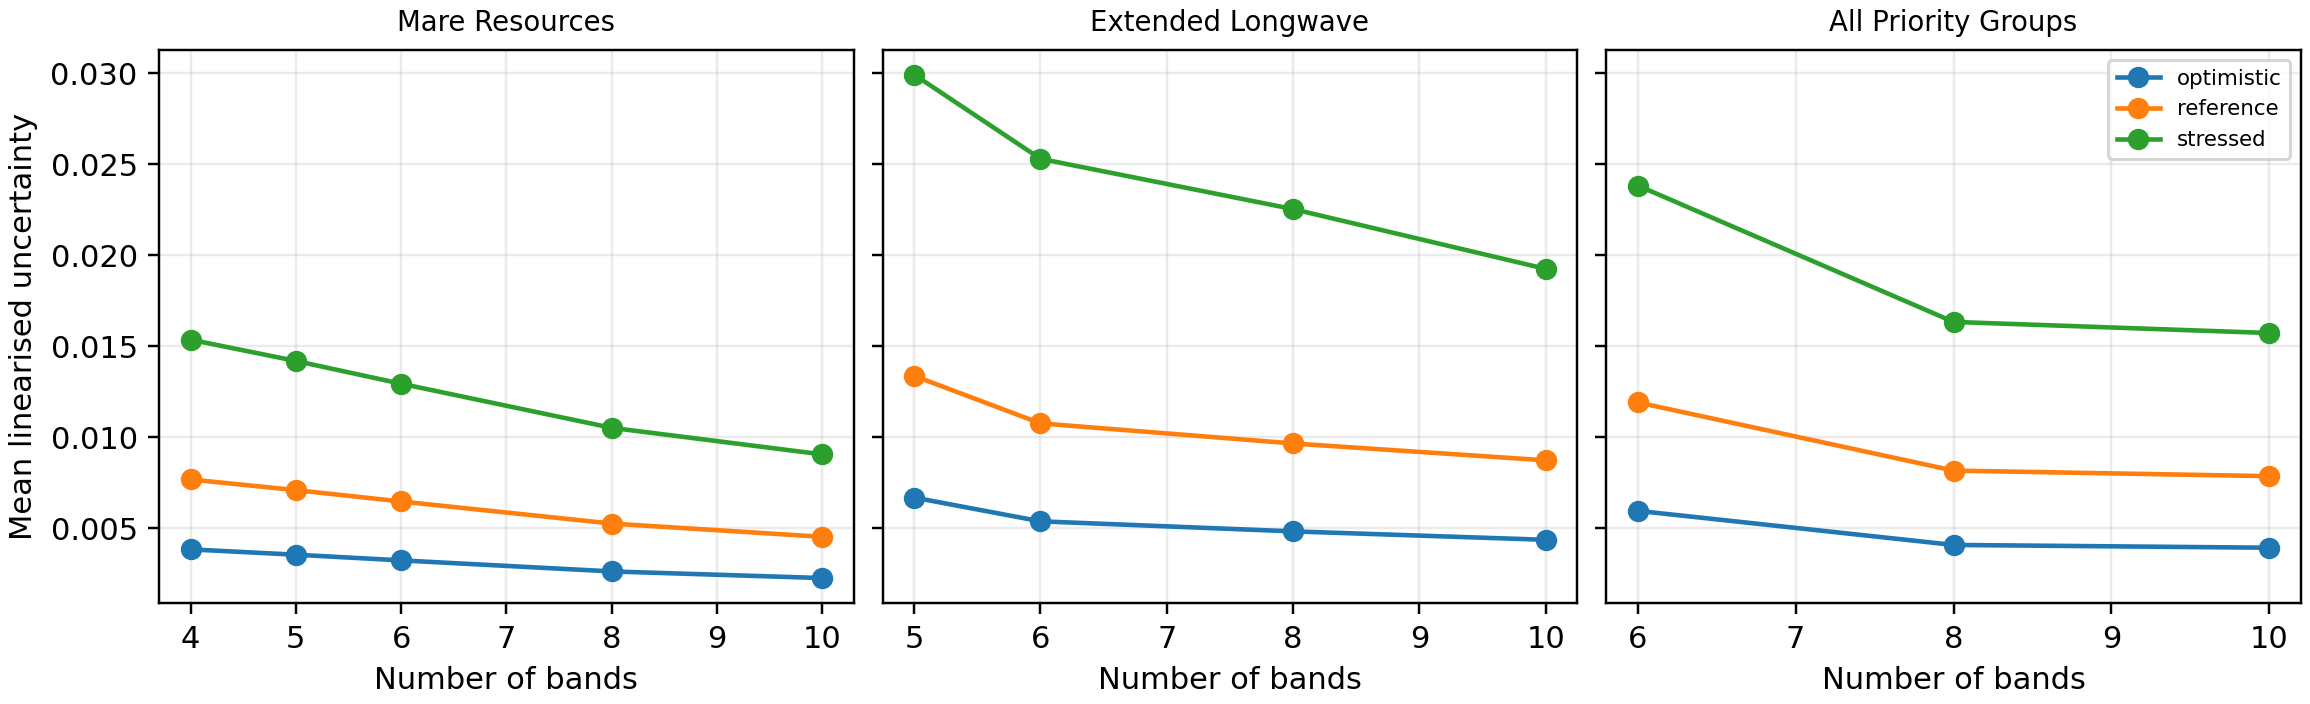
\includegraphics[width=\linewidth]{../outputs/figures/band_count_uncertainty.png}
\end{minipage}\hfill
\begin{minipage}[t]{0.49\textwidth}
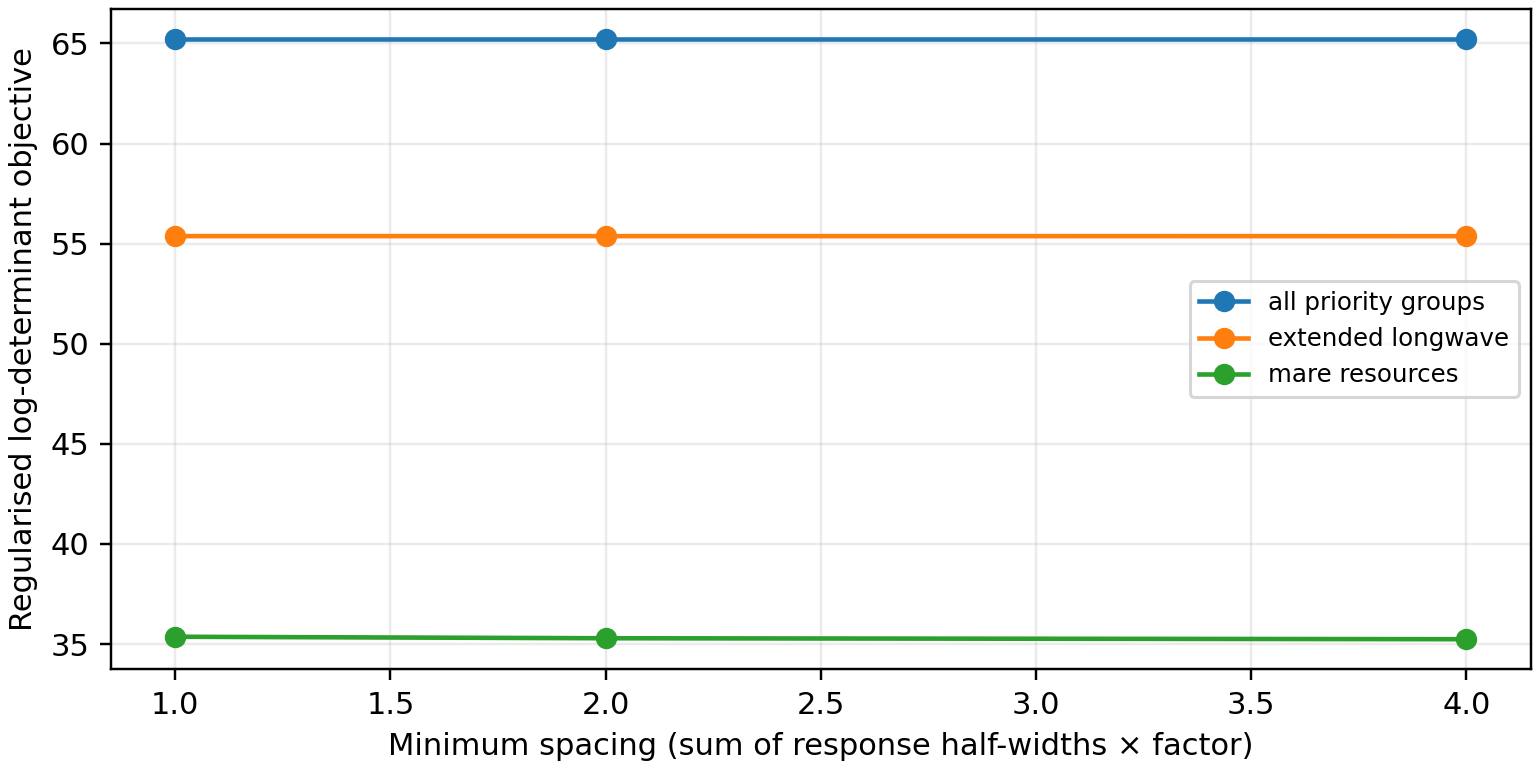
\includegraphics[width=\linewidth]{../outputs/figures/spacing_sensitivity.png}
\end{minipage}
\caption{Sensitivity to band count and assumed noise (left), and to the minimum separation of eight-band designs under reference noise (right). Infinite values caused by rank deficiency are omitted from the left plot. Spacing has little effect when the unconstrained choices are already separated; the mare case shows the largest, still modest, change.}
\label{fig:sensitivity}
\end{figure*}

The spacing sweep changes the eight-band information objective only weakly, demonstrating that the main solutions do not depend on densely packing adjacent FIR filters. In the mare case, the stricter constraint removes some closely placed VNIR candidates and causes a small objective loss. This is precisely why the constraint is exposed rather than hidden in one fixed minimum-distance number.

The signed objective difference between the greedy and genetic results was \MareGreedyGap\%, \LongwaveGreedyGap\%, and \AllGroupsGreedyGap\% for the mare, long-wave, and all-priority cases, respectively. Each negative value indicates a small improvement by the genetic search, which was seeded with the greedy solution. All improvements were below 0.2\%. This audit does not establish global optimality; it only shows that the two simple searches gave nearly equivalent objective values under the same assumptions.

Figure~\ref{fig:unmixing} gives the direct mixture test. Nominal RMSE is lowest for the four-component mare case and highest for the seven-group case. Calibration-only degradation remains limited, while combined stressed noise and mismatch approximately doubles or triples error. The full-group result is therefore useful as a baseline, but weaker than the smaller mission-specific configurations.

\begin{figure}[t]
\centering
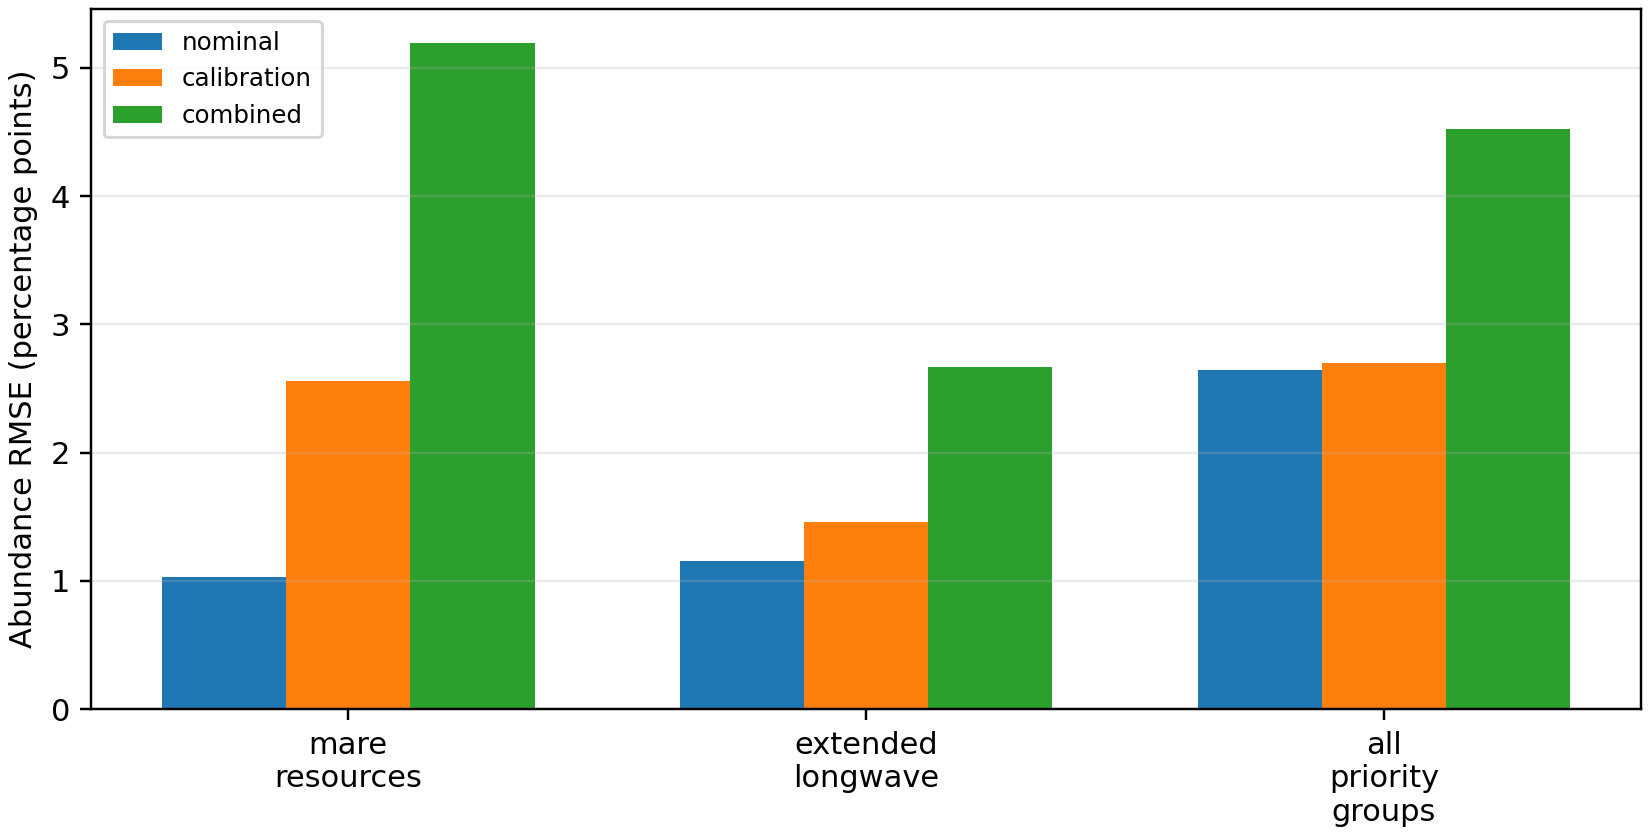
\includegraphics[width=\columnwidth]{../outputs/figures/unmixing_stress.png}
\caption{Empirical abundance RMSE for the selected reference configurations. ``Calibration'' adds band-centre and continuum mismatch at reference noise; ``combined'' also uses the stressed noise profile. These are controlled sensitivity cases, not confidence bounds for a flight instrument.}
\label{fig:unmixing}
\end{figure}

\section{Limitations}

The study is intentionally a baseline, and its limits define how the results may be used.

First, laboratory reflectance contrast is not at-sensor lunar radiance. A complete design requires illumination, surface temperature, emissivity, detector noise-equivalent radiance, optics, calibration, and viewing geometry. This is especially important beyond \SI{3}{\micro\metre}, where reflected and thermal contributions change with temperature. The adopted MIR noise and resolution values are transparent sensitivity assumptions, not validated hardware performance.

Second, linear mixtures and fixed composites omit intimate particulate mixing, multiple scattering, grain-size effects, glass and agglutinates, space weathering, temperature-dependent spectral shifts, and endmember variability \cite{hapke2012theory}. The continuum perturbation merely tests modest mismatch; it cannot be interpreted as a physical model of those processes. Similarly, room-condition RELAB spectra do not represent every lunar environmental state.

Third, the all-priority case retrieves seven functional groups, not 17 individual mineral abundances. Fewer than ten channels cannot generally identify 17 independent fractions. The grouping is appropriate only when the mission objective accepts class-level discrimination. Mineral-specific retrieval needs more bands, stronger priors, or a narrower target set.

Fourth, spectral support differs. Troilite, pyrrhotite, akaganeite, hematite, and the selected quartz measurements restrict relevant cases to approximately \SI{25}{\micro\metre}. They are not extrapolated to \SI{40}{\micro\metre}. The separate long-wave case demonstrates the full interval only for samples that actually cover it.

Finally, the study contains no spatial scene, orebody geometry, thermal model, or detection-probability calculation. It cannot substantiate a required ground-sampling distance or minimum detectable deposit. The greedy guarantee applies directly only to the cardinality-only objective, and the small genetic audit is not an exhaustive search. Results depend on the selected RELAB samples, grouping weights, response model, noise envelope, and simulated mixture distribution.

\section{Conclusion}

A short, reproducible method converts measured laboratory spectra into configuration-specific lunar spectral baselines. Three cases cover a compact mare example, a genuine 0.4--\SI{40}{\micro\metre} supported subset, and all 17 priority minerals as seven functional groups. Support auditing prevents artificial FIR bands; band-count, noise, and spacing sweeps show when a design becomes identifiable and how sensitive it is to engineering assumptions. Five bands support the simple mare example, while the broader grouped cases benefit from eight. Under the chosen synthetic mixtures, nominal errors remain at a few percentage points and rise clearly under combined stress. These values are useful for comparing concepts, not for claiming flight performance. The next defensible step is to replace the stated sensitivity envelopes with one instrument's radiance and calibration model, then test the bands on temperature- and grain-size-matched lunar analogue measurements.

\section*{Data and code availability}

The code, configurations, exact RELAB identifiers, checksums, machine-readable results, and figure-generation workflow are prepared in the companion repository at \url{https://github.com/XX}. The final archival DOI will be inserted as \texttt{XX} before submission. Original RELAB spectra remain subject to their source terms.

\section*{Acknowledgments}

The authors acknowledge Brown University RELAB and the lunar spectroscopy and instrument teams whose public measurements and publications support this study.

\balance
\bibliographystyle{unsrt}
\bibliography{references}
\end{document}
